In this section we evaluate the performance of the model as a function
of several important parameters. We focus in particular on how the
performance of the models changes as a function of the number of runs
included. From these evaluations, we conclude that (1) the model
performs well in its final form, (2) the model has reached a stable
state wherein inclusion of additional runs does not increase model
performance, and (3) the model is not over-fit to particular
experiments within a data set or to any data set as a whole.

\subsection{Comparison with other module detection algorithms}

We compared the number of \rdb~TFs detected in the \egrine~model to individual
\cm~runs as well as to several other module detection/clustering
algorithms that were computed on subsets of the experimental data
(similar to the \egrine~ensemble; Figure \ref{fig:motclust}). We
evaluated: (a) $k$-means clustering, (b) \tmsamp{WGCNA}
\cite{Langfelder2008}, and (c) \tmsamp{DISTILLER}
\cite{Lemmens2009}. For (a) and (b), we computed modules 100 times on
random subsets of the {\it E. coli} expression data set (using 200-250
randomly chosen experiments per run; selection criteria were identical
to {\it E. coli} \egrine; see Table~\ref{tab:cmparams:eco}). We then
predicted {\it de novo cis}-regulatory GREs in the promoter regions of genes
in each module using \tmsamp{MEME} (\tmsamp{MEME} parameters were also
identical to \egrine; Table~\ref{tab:cmparams:eco}). For (c), we
performed the comparison using the original modules generated by
\cite{Lemmens2009}. Rather than alter module composition by
re-detection, we instead varied \tmsamp{MEME} parameters applied to
the modules 100 times (again, within the same ranges as those used for
\egrine). TF-GRE matches were assigned by comparing GREs to
\rdb~TF binding sites, as previously described
(Section~\ref{section:tfbs:vs:regdb}).

We found that individual \cm~runs discovered a greater number of
\rdb~binding sites, on average, than the other methods (an average of
41 for \cm, compared to averages of 30, 25, and 29 for $k$-means,
\tmsamp{WGCNA}, and \tmsamp{DISTILLER}, respectively), which is
consistent with previous findings \cite{Reiss2006n}
(Figure~\ref{fig:ensemble_comparison_regDB}). Integration of all
\cm~biclusters into the complete \egrine~ensemble outperformed all
individual \cm~runs (53 total, as described in the Manuscript). This
result is typical of ensemble-based inference approaches, and supports
value of ensemble integration as part of the \egrine~ model.

\begin{figure}[h!]
\centering
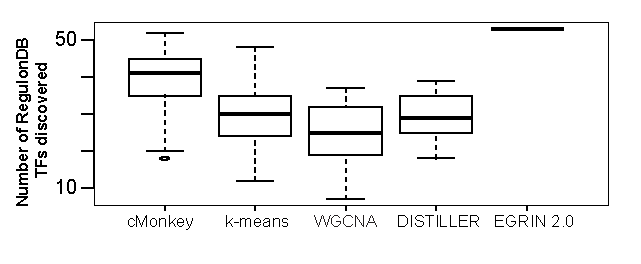
\includegraphics[width=0.95\linewidth]{figures/ensemble_comparison_regDB.pdf}
\caption[Number of TFs in \rdb~ re-discovered by various
    regulatory module detection methods.]  {{\bf Number of TFs in
    \rdb~ re-discovered by various regulatory module detection
    methods.} Comparison of \egrine~ (solid line, far right) to
  individual \cm\ runs, as well as multiple runs of $k$-means,
  \tmsamp{WGCNA}, and \tmsamp{DISTILLER} on subsets of the expression
  data. Evaluation made with respect to re-discovery of binding sites
  for 88 TFs with $\geq 3$ unique sites in \rdb~ based on genome-wide
  binding site locations (FDR $\leq 0.05$).}
\label{fig:ensemble_comparison_regDB}
\end{figure}

\subsection{Convergence and stability of the inferred network}

To evaluate the stability of the inferred \egrine network, we
quantified how the model changes as the underlying cMonkey models used
to construct the ensemble are altered. Since sub-bagging acts
similarly to cross-validation, we viewed this as an opportunity to
evaluate whether the model is over-fit to particular experiments in
the data set. Specifically, we asked how many runs are required to
converge on a consistently inferred network, i.e., where the inferred
gene-gene co-occurrence matrix is largely identical (see Section
\ref{}). In Figure \ref{fig:gBg_network_converge} we demonstrate
the. This means that even with

\begin{figure}[h!]
\centering
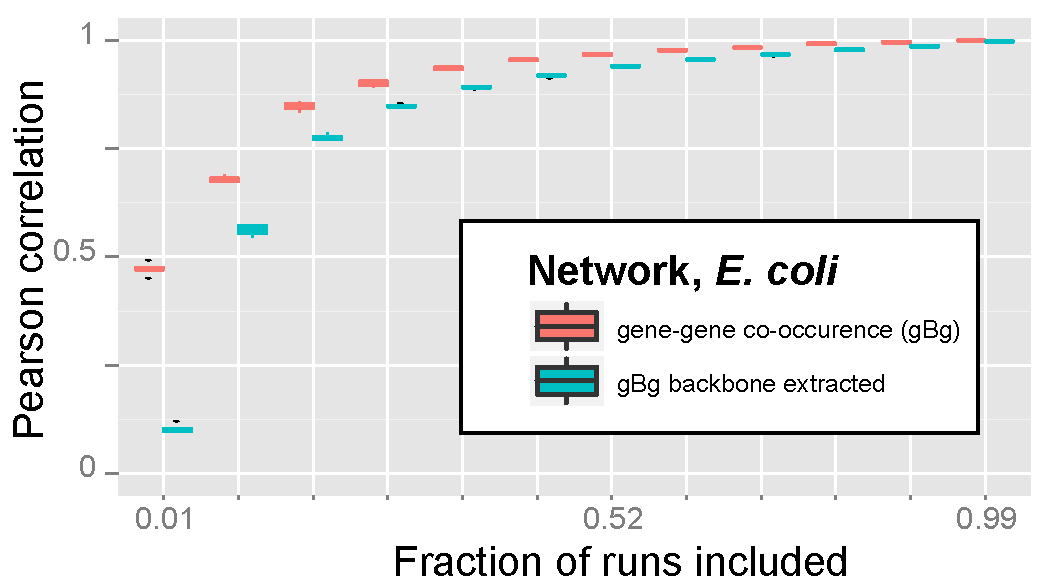
\includegraphics[width=0.75\linewidth]{figures/gBg_network_converge.pdf}
\caption[Convergence of \egrine inferred networks.]  {{\bf Convergence of \egrine inferred networks.}} 
\label{fig:gBg_network_converge}
\end{figure}

\subsection{Discovery of corems in an independent data set}

To determine whether the overfit 

\begin{figure}[h!]
\centering
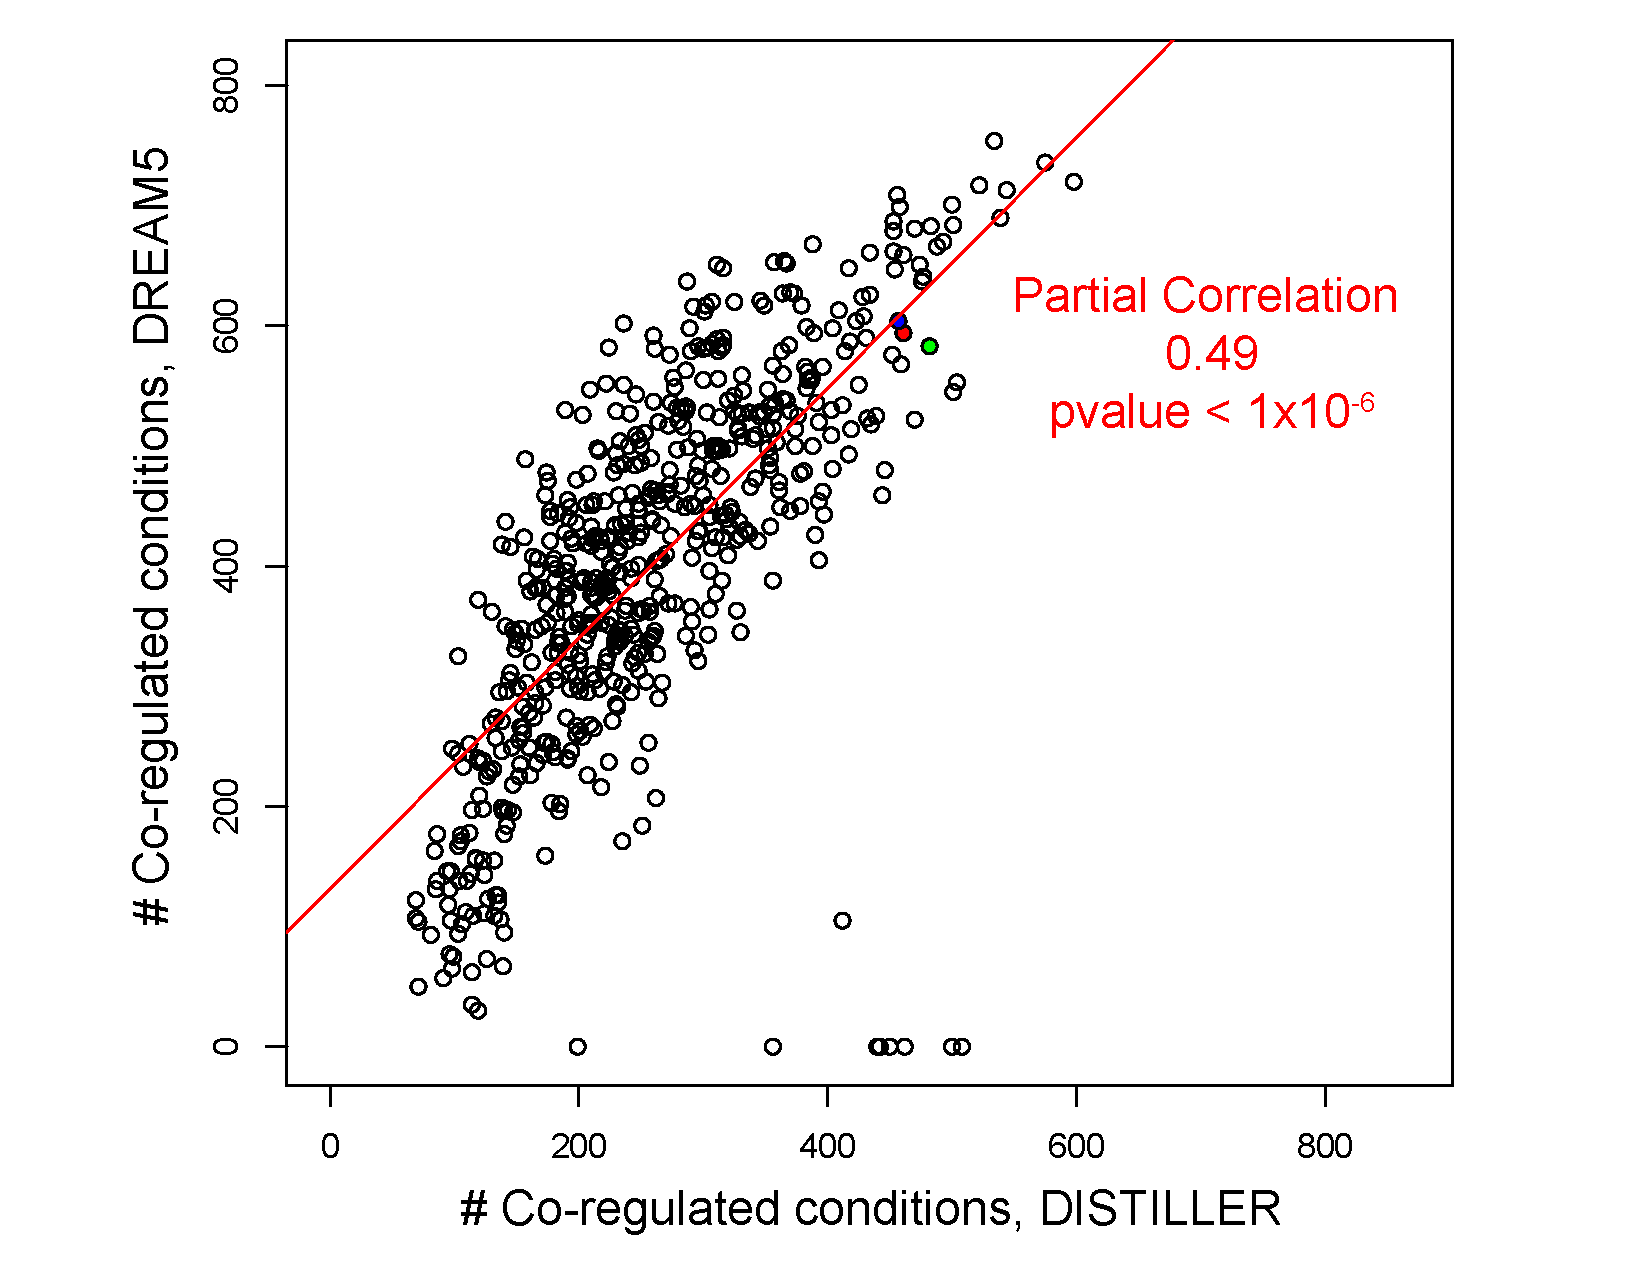
\includegraphics[width=0.75\linewidth]{figures/corem_conds_distiller_dream5.pdf}
\caption[Number of TFs in \rdb~ re-discovered by various
    regulatory module detection methods.]  {{\bf Number of TFs in
    \rdb~ re-discovered by various regulatory module detection
    methods.} Comparison of \egrine~ (solid line, far right) to
  individual \cm\ runs, as well as multiple runs of $k$-means,
  \tmsamp{WGCNA}, and \tmsamp{DISTILLER} on subsets of the expression
  data. Evaluation made with respect to re-discovery of binding sites
  for 88 TFs with $\geq 3$ unique sites in \rdb~ based on genome-wide
  binding site locations (FDR $\leq 0.05$).}
\label{fig:corem_conds_distiller_dream5}
\end{figure}

